\documentclass[11pt]{article}

\usepackage{october} \usepackage{lineno}
% For BJPS \hyphenpenalty=10000 \hbadness=10000

\begin{document}
% \setpagewiselinenumbers 
% \modulolinenumbers[5] 
% \linenumbers
% For BJPS \raggedright \doublespacing

% y=3;z=4;pdftk A=epsa-jeffrey-conditioning\ \($y\).pdf
% cat A1-$z output wc-out.pdf

% \title{Asymmetry and the Geometry of Reason} 
% \author{Anonymous}
% \date{}
% \maketitle
% \newcounter{expls} \doublespacing

\textbf{\Large Asymmetry and the Geometry of Reason}

\section{Introduction}
\label{intr}

The \qnull{geometry of reason} (a term coined by Richard Pettigrew and
Hannes Leitgeb, two of its advocates) refers to a view of epistemic
utility in which the underlying topology for credence functions (which
may be subjective probability distributions) on a finite number of
events is a metric space. This paper gives a detailed account how it
violates reasonable expectations for an acceptable model. A non-metric
alternative, information theory, fulfills many of these expectations
but violates others which are similarly intuitive.

There are several possibilities to deal with these violations: (i)
reject both the geometry of reason and information theory and provide
a third alternative; (ii) save one of the two accounts by weakening
the expectations and giving plausible explanations for these
weakenings, perhaps by providing a more advanced formal account; (iii)
provide an impossibility theorem that shows that no model can fulfill
all expectations. (iii) would favour some sort of pluralism. For (i),
I am not aware of a third alternative to the geometry of reason and
information theory. I favour possibility (ii). The model to save is
information theory and the advanced formal account is the theory of
differential manifolds. The problems for the geometry of reason are
irremediable. This paper, however, only reveals the seriousness and
extent of the violations, not the possible solutions.

I will assume probabilism and an isomorphism between probability
distributions $P$ on an outcome space $\Omega$ with $|\Omega|=n$ and
points $p\in\mathbb{S}^{n-1}\subset\mathbb{R}^{n}$ having coordinates
$p_{i}=P(\omega_{i}),i=1,\ldots,n$ and $\omega_{i}\in{}\Omega$. Since
the isomorphism is to a metric space, there is a distance relation
between credence functions which can be used to formulate axioms
relating credences to epistemic utility. For information theory, as
opposed to the geometry of reason, the underlying topology for
credence functions is not a metric space (see figures
\ref{fig:contourslp} and \ref{fig:contoursrj} for illustration).

\begin{figure}[ht]
  \begin{flushright}
    \begin{minipage}[h]{.7\linewidth}
      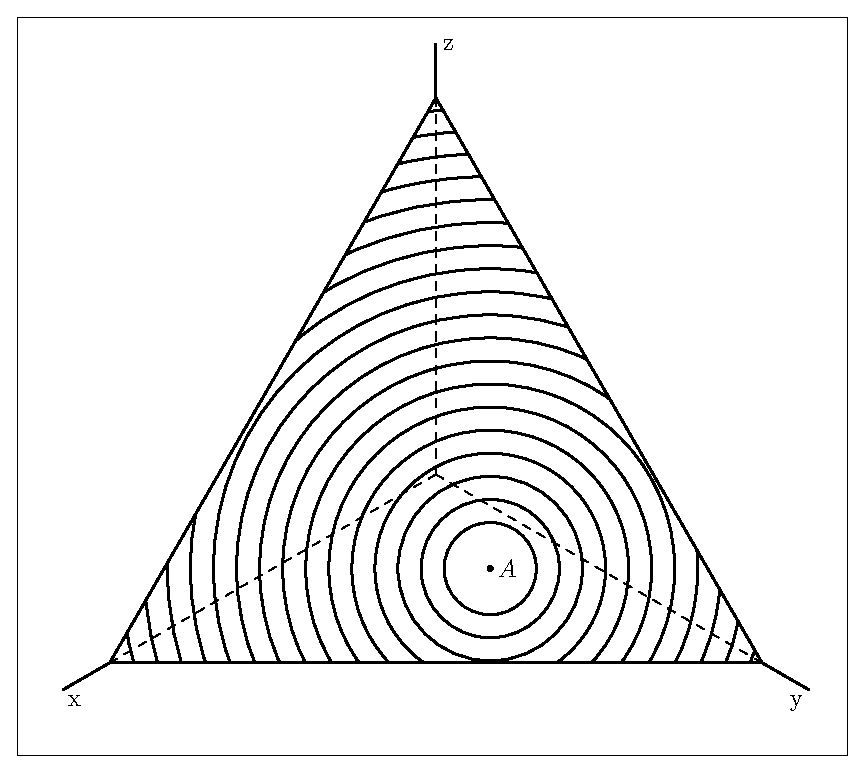
\includegraphics[width=\textwidth]{contourslp.eps}
      \caption{\footnotesize The simplex $\mathbb{S}^{2}$ in
        three-dimensional space $\mathbb{R}^{3}$ with contour lines
        corresponding to the geometry of reason around point $A$ in
        equation (\ref{eq:e6}). Points on the same contour line are
        equidistant from $A$ with respect to the Euclidean metric.
        Compare the contour lines here to figure \ref{fig:contoursrj}.
        Note that this diagram and all the following diagrams are
        frontal views of the simplex.}
      \label{fig:contourslp}
    \end{minipage}
  \end{flushright}
\end{figure}

\begin{figure}[ht]
  \begin{flushright}
    \begin{minipage}[h]{.7\linewidth}
      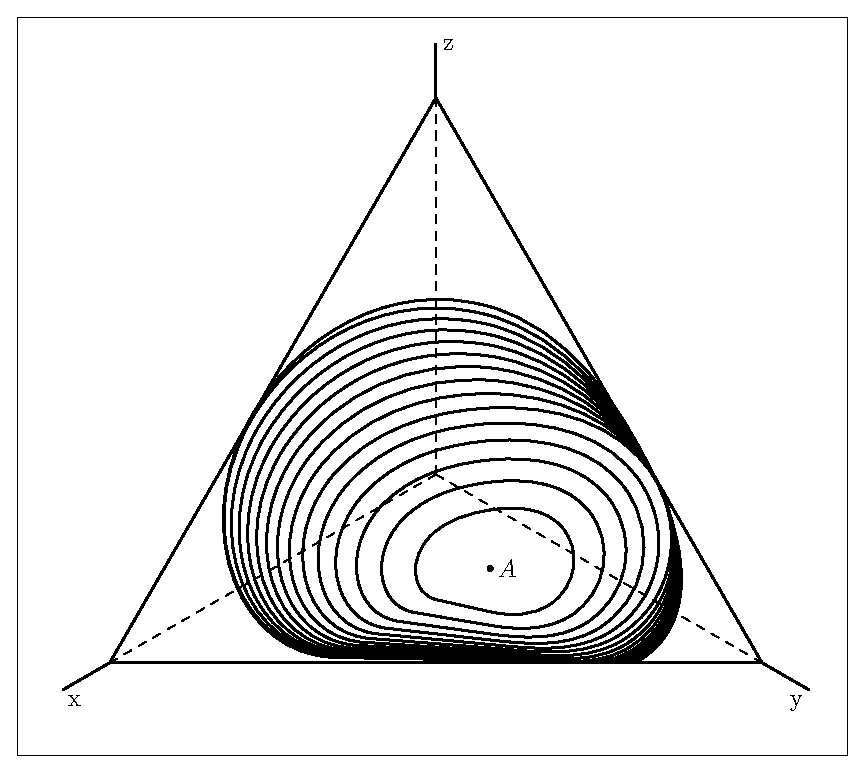
\includegraphics[width=\textwidth]{crj.eps}
      \caption{\footnotesize The simplex $\mathbb{S}^{2}$ with contour
        lines corresponding to information theory around point $A$ in
        equation (\ref{eq:e6}). Points on the same contour line are
        equidistant from $A$ with respect to the Kullback-Leibler
        divergence. The contrast to figure \ref{fig:contourslp} will
        become clear in much more detail in the body of the paper.
        Note that the contour lines of the geometry of reason are
        insensitive to the boundaries of the simplex, while the
        contour lines of information theory reflect them. One of the
        main arguments in this paper is that information theory
        respects epistemic intuitions we have about asymmetry:
        proximity to extreme beliefs with very high or very low
        probability influences the topology that is at the basis of
        updating.}
      \label{fig:contoursrj}
    \end{minipage}
  \end{flushright}
\end{figure}

I will show that LP conditioning, which is an alternative to Jeffrey
conditioning as a generalization of standard conditioning and which
the geometry of reason entails, fails commonsense expectations that
are reasonable to have for the kind of updating scenario that LP
conditioning addresses. Jeffrey conditioning fulfills these
commonsense expectations. Its failure to minimize inaccuracy on the
basis of the geometry of reason casts, by reductio, doubt on the
geometry of reason.

\begin{quotex}
  \beispiel{Sherlock Holmes}\label{ex:holmes} Sherlock Holmes
  attributes the following probabilities to the propositions $E_{i}$
  that $k_{i}$ is the culprit in a crime:
  $P(E_{1})=1/3,P(E_{2})=1/2,P(E_{3})=1/6$, where $k_{1}$ is Mr.\ R.,
  $k_{2}$ is Ms.\ S., and $k_{3}$ is Ms.\ T. Then Holmes finds some
  evidence which convinces him that $P'(F^{*})=1/2$, where $F^{*}$ is
  the proposition that the culprit is male and $P$ is relatively prior
  to $P'$. What should be Holmes' updated probability that Ms.\ S. is
  the culprit?
\end{quotex}

I will look at the recommendations of Jeffrey conditioning and LP
conditioning for {\xample} \ref{ex:holmes} in the next section. For
now note that LP conditioning violates all of the following plausible
expectations in List One\label{page:listone} for an amujus, an
\qnull{alternative method of updating for Jeffrey-type updating
  scenarios.} This is List One:

\begin{itemize}
\item \textsc{continuity} An amujus ought to be continuous with
  standard conditioning as a limiting case.
\item \textsc{regularity} An amujus ought not to assign a posterior
  probability of $0$ to an event which has a positive prior
  probability and about which the intervening evidence says nothing
  except that a strictly weaker event has a positive posterior
  probability.
\item \textsc{levinstein} An amujus ought not to give \qeins{extremely
    unattractive} results in a Levinstein scenario (see
  \scite{7}{levinstein12}{}, which not only articulates this failed
  expectation for LP conditioning, but also the previous two).
\item \textsc{invariance} An amujus ought to be partition invariant.
\item \textsc{expansibility} An amujus ought to be insensitive to an
  expansion of the event space by zero-probability events.
\item \textsc{confirmation} An amujus ought to align with intuitions
  we have about degrees of confirmation.
\item \textsc{horizon} An amujus ought to exhibit the horizon effect
  which makes probability distributions which are nearer to extreme
  probability distributions appear to be closer to each other than
  they really are.
\end{itemize}

Jeffrey conditioning and LP conditioning are both an amujus based on a
concept of quantitative difference between probability distributions
measured as a function on the isomorphic manifold (in our case, an
$n-1$-dimensional simplex). Evidence appears in the form of a
constraint on acceptable probability distributions and the closest
acceptable probability to the orginal (relatively prior) probability
distribution is chosen as its successor. Here is List
Two\label{page:listtwo}, a list of reasonable expectations one may
have toward this concept of quantitative difference (we call it a
distance function for the geometry of reason and a divergence for
information theory). Let $d(p,q)$ express this concept mathematically.

\begin{itemize}
\item \textsc{triangularity} The concept obeys the triangle
  inequality. If there is an intermediate probability distribution, it
  will not make the difference smaller: $d(p,r)\leq{}d(p,q)+d(q,r)$.
  Buying a pair of shoes is not going to be more expensive than buying
  the two shoes individually.
\item \textsc{collinear horizon} This expecation is just a more
  technical restatement of the \textsc{horizon} expectation in the
  previous list. If $p,p',q,q'$ are collinear with the centre of the
  simplex $m$ (whose coordinates are $m_{i}=1/n$ for all $i$) and an
  arbitrary but fixed boundary point $\xi\in\partial\mathbb{S}^{n-1}$
  and $p,p',q,q'$ are all between $m$ and $\xi$ with
  $\|p'-p\|=\|q'-q\|$ where $p$ is strictly closest to $m$, then
  $|d(p,p')|<|d(q,q')|$. For an illustration of this expectation see
  figure \ref{fig:conditions}. The absolute value is added as a
  feature to accommodate degree of confirmation functions in
  subsection \ref{Confirmation}, which may be negative.
\item \textsc{transitivity of asymmetry} An ordered pair $(p,q)$ of
  simplex points associated with probability distributions is
  asymmetrically negative, positive, or balanced, so either
  $d(p,q)-d(q,p)<0$ or $d(p,q)-d(q,p)>0$ or $d(p,q)-d(q,p)=0$. If
  $(p,q)$ and $(q,r)$ are asymmetrically positive, $(p,r)$ ought not
  to be asymmetrically negative. Think of a bicycle route map with
  different locations at varying altitudes. If it takes 20 minutes to
  get from $A$ to $B$ but only 15 minutes to get from $B$ to $A$ then
  $(A,B)$ is asymmetrically positive. If $(A,B)$ and $(B,C)$ are
  asymmetrically positive, then $(A,C)$ ought not to be asymmetrically
  negative.
\end{itemize}

\begin{figure}[ht]
  \begin{flushright}
    \begin{minipage}[h]{.7\linewidth}
      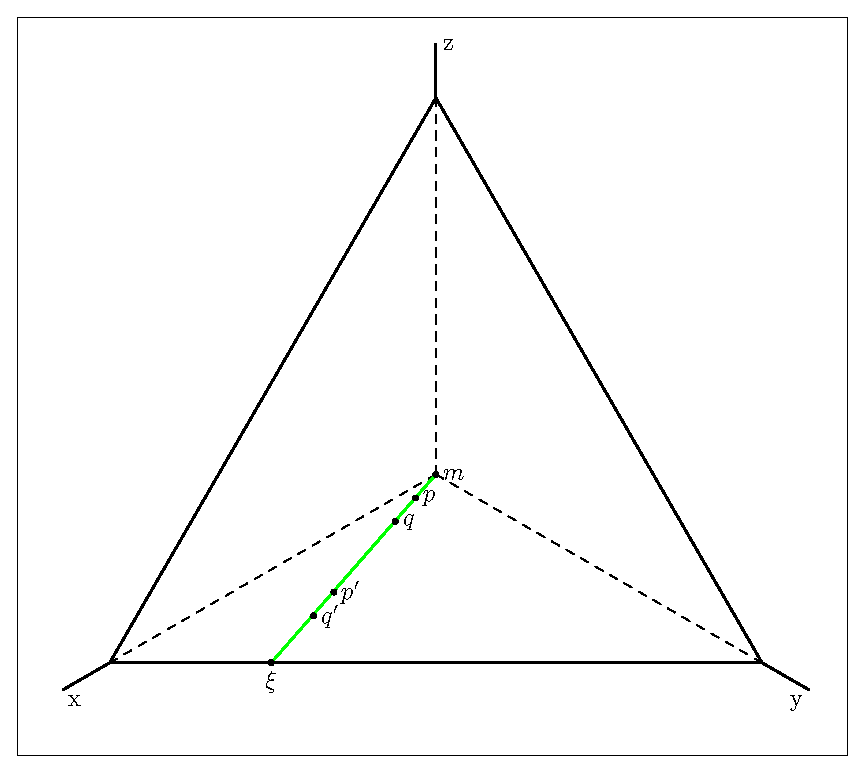
\includegraphics[width=\textwidth]{horeff.eps}
      \caption{\footnotesize An illustrations of conditions (i)--(iii)
        for \textsc{collinear horizon} in List Two. $p,p'$ and $q,q'$
        must be equidistant and collinear with $m$ and $\xi$. If
        $q,q'$ is more peripheral than $p,p'$, then \textsc{collinear
          horizon} requires that $|d(p,p')|<|d(q,q')|$.}
      \label{fig:conditions}
    \end{minipage}
  \end{flushright}
\end{figure}

While the Kullback-Leibler divergence of information theory fulfills
all the expectations of List One, save \textsc{horizon}, it fails all
the expectations in List Two. Obversely, the Euclidean distance of the
geometry of reason fulfills all the expectations of List Two, save
\textsc{collinear horizon}, and fails all the expectations in List
One.

\section{Geometry of Reason versus Information Theory}
\label{grit}

Consider the following three points in three-dimensional space:

\begin{equation}
  \label{eq:e6}
  a=\left(\frac{1}{3},\frac{1}{2},\frac{1}{6}\right) \hspace{.5in}
  b=\left(\frac{1}{2},\frac{3}{8},\frac{1}{8}\right)  \hspace{.5in}
  c=\left(\frac{1}{2},\frac{5}{12},\frac{1}{12}\right)
\end{equation}

All three are elements of the simplex $\mathbb{S}^{2}$: their
coordinates add up to $1$. Thus they represent probability
distributions $A,B,C$ over a partition of the event space into three
events. Now call $D_{\mbox{\tiny KL}}(B,A)$ the Kullback-Leibler
divergence of $B$ from $A$ defined as follows, where $a_{i}$ are the
Cartesian coordinates of $a$:

\begin{equation}
  \label{eq:e7}
  D_{\mbox{\tiny KL}}(B,A)=\sum_{i=1}^{3}b_{i}\log\frac{b_{i}}{a_{i}}.
\end{equation}

Note that the Kullback-Leibler divergence, irrespective of dimension,
is always positive as a consequence of Gibbs' inequality (see
\scite{7}{mackay03}{}, sections 2.6 and 2.7).

Let the Euclidean distance $\|B-A\|$ be defined as usual by
$\sqrt{\sum_{i=1}^{n}\left(b_{i}-a_{i}\right)^{2}}$. What is
remarkable about the three points in (\ref{eq:e6}) is that

\begin{equation}
  \label{eq:e8}
  \|C-A\|\approx{}0.204<\|B-A\|\approx{}0.212
\end{equation}

and

\begin{equation}
  \label{eq:e9}
  D_{\mbox{\tiny KL}}(B,A)\approx{}0.0589<D_{\mbox{\tiny KL}}(C,A)\approx{}0.069.
\end{equation}

The Kullback-Leibler divergence and Euclidean distance give different
re\-commendations with respect to proximity. Let me explain how this
ties in with Jeffrey conditioning and LP conditioning.

\begin{figure}[ht]
  \begin{flushright}
    \begin{minipage}[h]{.7\linewidth}
      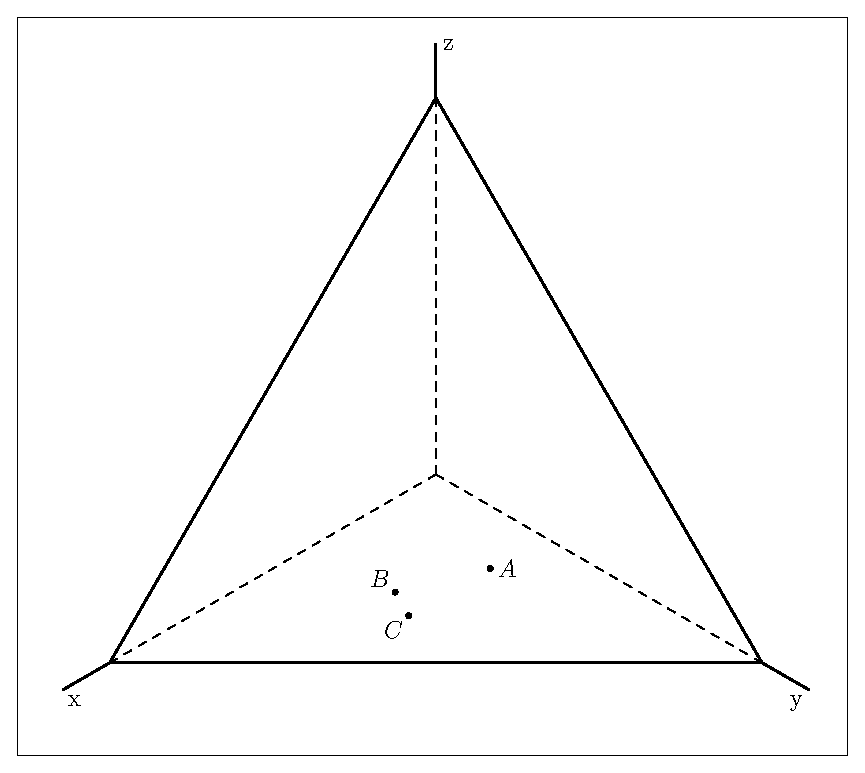
\includegraphics[width=\textwidth]{threepoints.eps}
      \caption{\footnotesize The simplex $\mathbb{S}^{2}$ in
        three-dimensional space $\mathbb{R}^{3}$ with points $a,b,c$
        as in equation (\ref{eq:e6}) representing probability
        distributions $A,B,C$. Note that geometrically speaking $C$ is
        closer to $A$ than $B$ is. Using the Kullback-Leibler
        divergence, however, $B$ is closer to $A$ than $C$ is.}
      \label{fig:threepoints}
    \end{minipage}
  \end{flushright}
\end{figure}

\begin{quotex}
  \beispiel{Abstract Holmes}\label{ex:abstract} Consider a possibility
  space $W=E_{1}\cup{}E_{2}\cup{}E_{3}$ (the $E_{i}$ are sets of
  states which are pairwise disjoint and whose union is $W$) and a
  partition $\mathcal{F}$ of $W$ such that
  $\mathcal{F}=\{F^{*},F^{**}\}=\{E_{1},E_{2}\cup{}E_{3}\}$.
\end{quotex}

Let $P$ be the prior probability function on $W$ and $P'$ the
posterior. I will keep the notation informal to make this simple.
Jeffrey-type updating scenarios give us new information on the
posterior probabilities of partitions such as $\mathcal{F}$. In
{\xample} \ref{ex:abstract}, let

\begin{equation}
  \label{eq:priors}
  \begin{array}{rcl}
    P(E_{1})&=&1/3 \\
    P(E_{2})&=&1/2 \\
    P(E_{3})&=&1/6
  \end{array}
\end{equation}

and the new evidence constrain $P'$ such that
$P'(F^{*})=1/2=P'(F^{**})$.

Jeffrey conditioning works on the intuition that the posterior
probabilities conditional on the partition elements equal their
priors. Hence,

\begin{align}
  \label{eq:jc}
  &P'_{\mbox{\tiny JC}}(E_{i})&=&P'(E_{i}|F^{*})P'(F^{*})+P'(E_{i}|F^{**})P'(F^{**})\notag \\
  &&=&P(E_{i}|F^{*})P'(F^{*})+P(E_{i}|F^{**})P'(F^{**})
\end{align}

Leitgeb and Pettigrew introduce an alternative to Jeffrey
conditioning, which we have called LP conditioning. It proceeds as
follows for {\xample} \ref{ex:abstract} and in general provides the
minimally inaccurate posterior probability distribution in
Jeffrey-type updating scenarios.

Solve the following two equations for $x$ and $y$:

\begin{equation}
  \label{eq:lpce}
  \begin{array}{rcl}
    P(E_{1})+x&=&P'(F^{*}) \\
    P(E_{2})+y+P(E_{3})+y&=&P'(F^{**})
  \end{array}
\end{equation}

and then set

\begin{equation}
  \label{eq:lpcf}
  \begin{array}{rcl}
    P'_{\mbox{\tiny LP}}(E_{1})&=&P(E_{1})+x \\
    P'_{\mbox{\tiny LP}}(E_{2})&=&P(E_{2})+y \\
    P'_{\mbox{\tiny LP}}(E_{3})&=&P(E_{3})+y
  \end{array}
\end{equation}

For the more formal and more general account see
\scite{8}{leitgebpettigrew10ii}{254}. The results for {\xample}
\ref{ex:abstract} are:

\begin{equation}
  \label{eq:lpcres}
  \begin{array}{rcl}
    P'_{\mbox{\tiny LP}}(E_{1})&=&1/2 \\
    P'_{\mbox{\tiny LP}}(E_{2})&=&5/12 \\
    P'_{\mbox{\tiny LP}}(E_{3})&=&1/12
  \end{array}
\end{equation}

Compare these results to the results of Jeffrey conditioning:

\begin{equation}
  \label{eq:jcres}
  \begin{array}{rcl}
    P'_{\mbox{\tiny JC}}(E_{1})&=&1/2 \\
    P'_{\mbox{\tiny JC}}(E_{2})&=&3/8 \\
    P'_{\mbox{\tiny JC}}(E_{3})&=&1/8
  \end{array}
\end{equation}

Note that (\ref{eq:priors}), (\ref{eq:jcres}), and (\ref{eq:lpcres})
correspond to $A,B,C$ in (\ref{eq:e6}).

\section{Expectations for the Geometry of Reason}
\label{fivex}

It remains to provide more detail for the expectations in List One
(see page \pageref{page:listone}) and to show how LP conditioning
violates them. These subsections have been abridged to accommodate the
word limit for this submission. The full-length paper contains the
complete version of these arguments, especially their formal
components and examples.

\subsection{Continuity}
\label{Continuity}

LP conditioning violates \textsc{continuity} because standard
conditioning gives a different recommendation than a parallel sequence
of Jeffrey-type updating scenarios which get arbitrarily close to
standard event observation. This is especially troubling considering
how important the case for standard conditioning is to Leitgeb and
Pettigrew.

\subsection{Regularity}
\label{Regularity}

LP conditioning violates \textsc{regularity} because formerly positive
probabilities can be reduced to $0$ even though the new information in
the Jeffrey-type updating scenario makes no such requirements (as is
usually the case for standard conditioning). Ironically, Jeffrey-type
updating scenarios are meant to be a better reflection of real-life
updating because they avoid extreme probabilities.

The violation becomes serious if we are already sympathetic to an
infor\-ma\-tion-based account: the amount of information required to
turn a non-extreme probability into one that is extreme ($0$ or $1$)
is infinite. Whereas the geometry of reason considers extreme
probabilities to be easily accessible by non-extreme probabilities
under new information (much like a marble rolling off a table or a
bowling ball heading for the gutter), information theory envisions
extreme probabilities more like an event horizon. The nearer you are
to the extreme probabilities, the more information you need to move
on. For an observer, the horizon is never reached.

\subsection{Levinstein}
\label{Levinstein}

LP conditioning violates \textsc{levinstein} because of \qeins{the
  potentially dramatic effect [LP conditioning] can have on the
  likelihood ratios between different propositions}
\scite{3}{levinstein12}{419}. Levinstein proposes a logarithmic
inaccuracy measure as a remedy to avoid violation of
\textsc{levinstein}. As a special case of applying a Levinstein-type
logarithmic inaccuracy measure, information theory does not violate
\textsc{levinstein}.

\subsection{Invariance}
\label{Invariance}

LP conditioning violates \textsc{invariance} because two agents who
have identical credences with respect to a partition of the event
space may disagree about this partition after LP conditioning, even
when the Jeffrey-type updating scenario provides no new information
about the more finely grained partitions on which the two agents
disagree.

\subsection{Expansibility}
\label{Expansibility}

One particular problem with the lack of invariance for LP conditioning
is how zero-probability events should be included in the list of prior
probabilities that determines the value of the posterior
probabilities. Consider

\begin{equation}
  \label{eq:reginvone}
  \begin{array}{rcl}
    P(X_{1})&=&0\\
    P(X_{2})&=&0.3\\
    P(X_{3})&=&0.6\\
    P(X_{4})&=&0.1\\
  \end{array}
\end{equation}

That $P(X_{1})=0$ may be a consequence of standard conditioning in a
previous step. Now the agent learns that $P'(X_{3}\vee{}X_{4})=0.5$.
Should the agent update on the list presented in (\ref{eq:reginvone})
or on the following list:

\begin{equation}
  \label{eq:reginvtwo}
  \begin{array}{rcl}
    P(X_{2})&=&0.3\\
    P(X_{3})&=&0.6\\
    P(X_{4})&=&0.1\\
  \end{array}
\end{equation}

Whether you update on (\ref{eq:reginvone}) or (\ref{eq:reginvtwo})
makes no difference to Jeffrey conditioning, but due to the lack of
invariance it makes a difference to LP conditioning, so the geometry
of reason needs to find a principled way to specify the appropriate
prior probabilities. 

\subsection{Horizon}
\label{Horizon}

It ought to be more difficult to update as probabilities become more
extreme (or less middling). I have formalized this requirement in List
Two (see page \pageref{page:listtwo}). It is trivial that the geometry
of reason does not fulfill it. Information theory fails as well, which
gives the horizon effect its prominent place in both lists. The way
information theory fails, however, is quite different. Near the
boundary of $\mathbb{S}^{n-1}$, information theory reflects the
horizon effect just as our expectation requires. The problem is near
the centre, where some equidistant points are more divergent the
closer they are to the middle. I will give an example and more
explanation in subsection \ref{subsec:colhor}.

\subsection{Confirmation}
\label{Confirmation}

This is a lengthy subsection and has been cut from the submission in
order to accommodate the word limit for this submission. Although it
contributes an interesting perspective to the problem, it is not
essential to my claims.

\section{Expectations for Information Theory}
\label{sec:expinfth}

In information theory, the information loss differs depending on
whether one uses probability distribution $P$ to encode a message
distributed according to probability distribution $Q$, or whether one
uses probability distribution $Q$ to encode a message distributed
according to probability distribution $P$. This asymmetry may very
well carry over into the epistemic realm. Updating from one
probability distribution, for example, which has $P(X)=x>0$ to
$P'(X)=0$ is common. It is called standard conditioning. Going in the
opposite direction, however, from $P(X)=0$ to $P'(X)=x'>0$ is
controversial and unusual.

The Kullback-Leibler divergence, which is the most promising concept
of difference for probability distributions in information theory and
the one which gives us Bayesian standard conditioning as well as
Jeffrey conditioning, is non-commutative and may provide the kind of
asymmetry required to reflect epistemic asymmetry. However, it also
violates \textsc{triangularity}, \textsc{collinear horizon}, and
\textsc{transitivity of asymmetry}. The task of this section is to
show how serious these violations are.

\subsection{Triangularity}
\label{subsec:triangularity}

The three points $A,B,C$ in (\ref{eq:e6}) violate
\textsc{triangularity}:

\begin{equation}
  \label{eq:yohliimo}
  D_{\mbox{\tiny KL}}(A,C)>D_{\mbox{\tiny KL}}(B,C)+D_{\mbox{\tiny KL}}(A,B).
\end{equation}

This is counterintuitive on a number of levels, some of which I have
already hinted at in illustration: taking a shortcut while making a
detour; buying a pair of shoes for more money than buying the shoes
individually.

Information theory violates \textsc{triangularity} in a particularly
egregious way. Consider any distinct two points $x$ and $z$ on
$\mathbb{S}^{n-1}$ with coordinates $x_{i}$ and $z_{i}$
($1\leq{}i\leq{}n$). For simplicity, let us write
$\delta(x,z)=D_{\mbox{\tiny KL}}(z,x)$. Then, for any
$\vartheta\in{}(0,1)$ and an intermediate point $y$ with coordinates
$y_{i}=\vartheta{}x_{i}+(1-\vartheta)z_{i}$, the following inequality
holds true:

\begin{equation}
  \label{eq:aiphedau}
  \delta(x,z)>\delta\left(x,y\right)+\delta\left(y,z\right).
\end{equation}

To prove this it is straightforward to see that (\ref{eq:aiphedau}) is
equivalent to

\begin{equation}
  \label{eq:eiquotoh}
  \sum_{i=1}^{n}(z_{i}-x_{i})\log\frac{\vartheta{}x_{i}+(1-\vartheta)z_{i}}{x_{i}}>0.
\end{equation}

Now we use the following trick. Expand the right hand side to

\begin{equation}
  \label{eq:xiechuth}
  \sum_{i=1}^{n}\left(z_{i}+\frac{\vartheta}{1-\vartheta}x_{i}-\frac{\vartheta}{1-\vartheta}x_{i}-x_{i}\right)\log\frac{\frac{1}{1-\vartheta}\left(\vartheta{}x_{i}+(1-\vartheta)z_{i}\right)}{\frac{1}{1-\vartheta}x_{i}}>0.
\end{equation}

(\ref{eq:xiechuth}) is clearly equivalent to (\ref{eq:eiquotoh}). It
is also equivalent to

\begin{equation}
  \label{eq:ohrohshi}
  \sum_{i=1}^{n}\left(z_{i}+\frac{\vartheta}{1-\vartheta}x_{i}\right)\log\frac{z_{i}+\frac{\vartheta}{1-\vartheta}x_{i}}{\frac{1}{1-\vartheta}x_{i}}+
  \sum_{i=1}^{n}\frac{1}{1-\vartheta}x_{i}\log\frac{\frac{1}{1-\vartheta}x_{i}}{z_{i}+\frac{\vartheta}{1-\vartheta}x_{i}}>0,
\end{equation}

which is true by Gibbs' inequality.
% (see \scite{7}{mackay03}{}, section 2.6 and 2.7).

\subsection{Collinear Horizon}
\label{subsec:colhor}

Here is a simple example.

\begin{equation}
  \label{eq:ubiesohx}
  p=\left(\frac{1}{5},\frac{2}{5},\frac{2}{5}\right) \hspace{.5in}
  p'=q=\left(\frac{1}{4},\frac{3}{8},\frac{3}{8}\right)  \hspace{.5in}
  q'=\left(\frac{3}{10},\frac{7}{20},\frac{7}{20}\right)
\end{equation}

The conditions of \textsc{collinear horizon} in List Two (see page
\pageref{page:listtwo}) are fulfilled. If $p$ represents $A$, $p'$ and
$q$ represent $B$, and $q'$ represents $C$, then note that
$\|b-a\|=\|c-b\|$ and $m,a,b,c$ are collinear. In violation of
\textsc{collinear horizon},

\begin{equation}
  \label{eq:eiloothu}
  D_{\mbox{\tiny KL}}(B,A)=7.3820\cdot{}10^{-3}>6.4015\cdot{}10^{-3}=D_{\mbox{\tiny KL}}(C,B).
\end{equation}

The bitter aftertaste that remains with \textsc{collinear horizon} is
that it is opaque what motivates information theory not only to put
probability distributions farther apart near the periphery, as I would
expect, but also near the centre. I lack the epistemic intuition
reflected in this behaviour.

\subsection{Transitivity of Asymmetry}
\label{subsec:Asymmetry}

Asymmetry presents a problem for the geometry of reason as well as for
information theory. For the geometry of reason, the problem is akin to
\textsc{continuity}. For information theory, the problem is the
non-trivial nature of the asymmetries it induces, which somehow need
to be reconnected to epistemic justification. 

Extreme probabilities are special and create asymmetries in updating:
moving in direction from certainty to uncertainty is asymmetrical to
moving in direction from uncertainty to certainty. Geometry of
reason's metric topology, however, allows for no asymmetries.

Now consider information theory. Given the asymmetric similarity
measure of probability distributions that information theory requires
(the Kullback-Leibler divergence), a prior probability distribution
$P$ may be closer to a posterior probability distribution $Q$ than $Q$
is to $P$ if their roles (prior-posterior) are reversed. That is just
what we would expect. The problem is that there is another posterior
probability distribution $R$ where the situation is just the opposite:
prior $P$ is further away from posterior $R$ than prior $R$ is from
posterior $P$. And whether a probability distribution different from
$P$ is of the $Q$-type or of the $R$-type escapes any epistemic
intuition.

For simplicity, let us look at probability distributions and their
associated credence functions on an event space with three atoms
$\Omega=\{\omega_{1},\omega_{2},\omega_{3}\}$. The simplex
$\mathbb{S}^{2}$ represents all of these probability distributions.
Every point $p$ in $\mathbb{S}^{2}$ representing a probability
distribution $P$ induces a partition on $\mathbb{S}^{2}$ into points
that are symmetric to $p$, positively skew-symmetric to $p$, and
negatively skew-symmetric to $p$ given the topology of information
theory.

In other words, if

\begin{equation}
  \label{eq:sksy}
  \Delta_{P}(P')=D_{\mbox{\tiny KL}}(P',P)-D_{\mbox{\tiny KL}}(P,P'),
\end{equation}

then, holding $P$ fixed, $\mathbb{S}^{2}$ is partitioned into three
regions,

\begin{equation}
  \label{eq:sieruxis}
  \Delta^{-1}(\mathbb{R}_{>0})\hspace{.5in}\Delta^{-1}(\mathbb{R}_{<0})\hspace{.5in}\Delta^{-1}(\{0\})
\end{equation}

\begin{figure}[ht]
  \begin{flushright}
    \begin{minipage}[h]{\linewidth}
      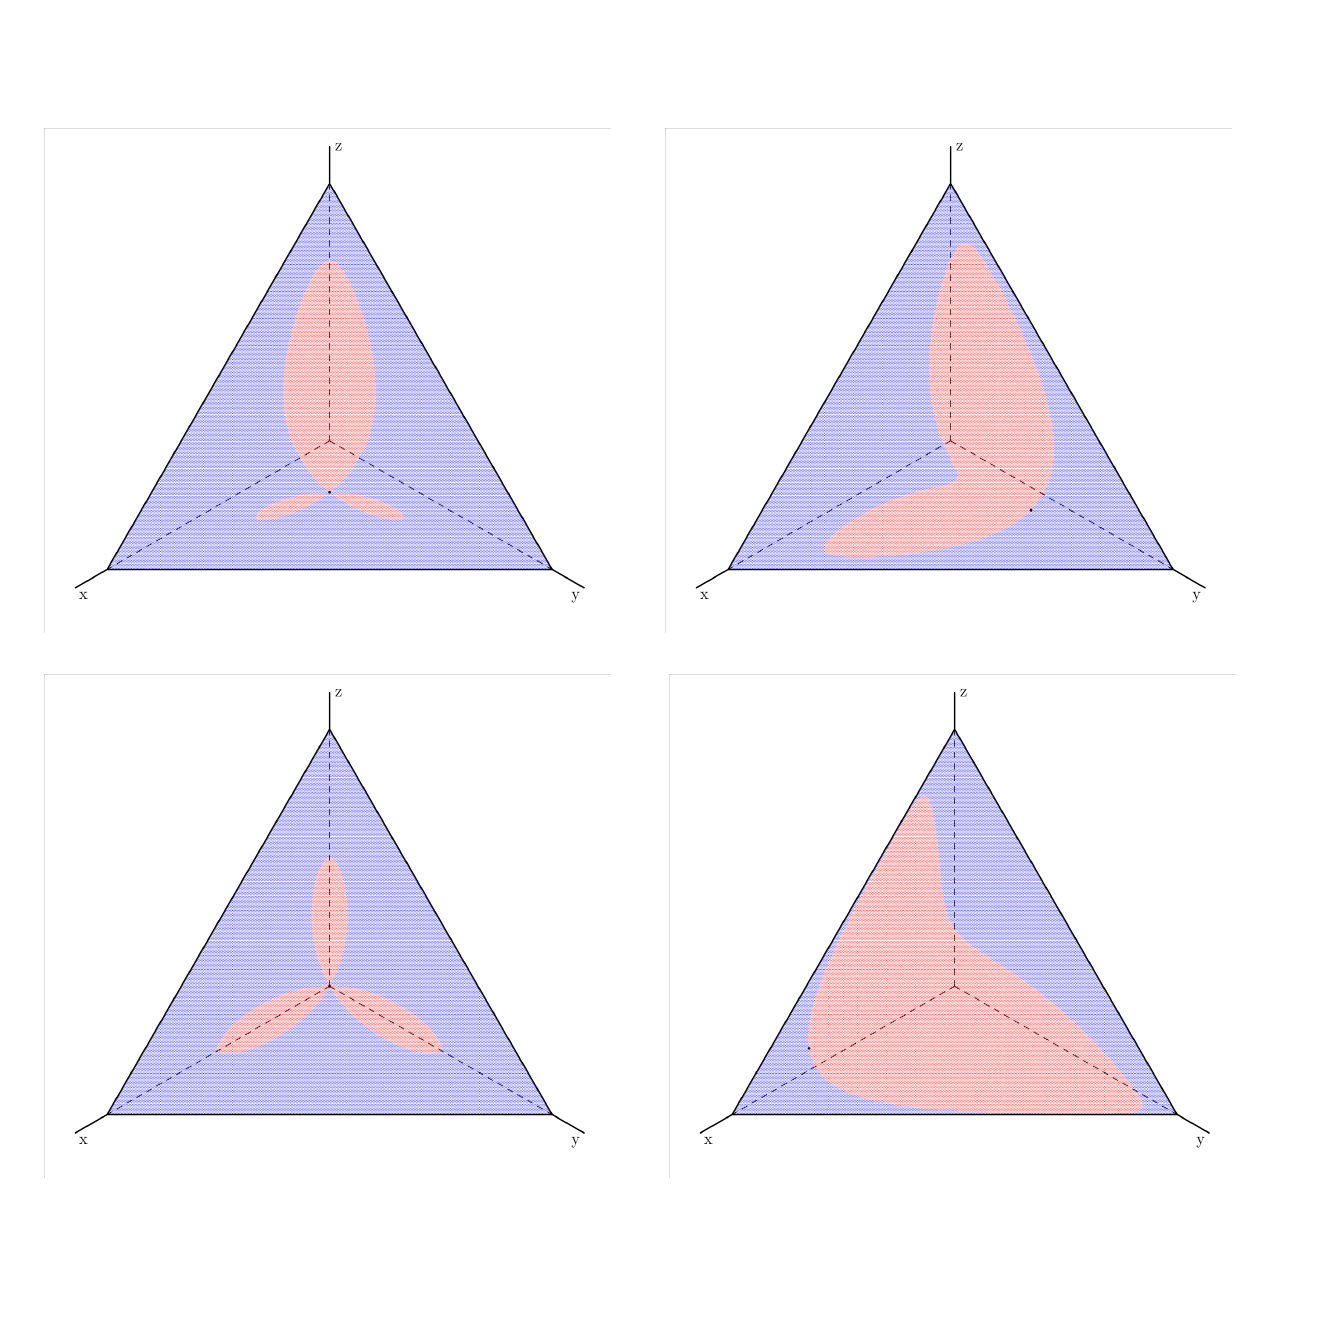
\includegraphics[width=\textwidth]{concat2.png}
      \caption{\footnotesize The partition (\ref{eq:sieruxis}) based
        on different values for $P$. From top left to bottom right,
        $P=(0.4,0.4,0.2); P=(0.242,0.604,0.154); P=(1/3,1/3,1/3);
        P=(0.741,0.087,0.172)$.
        Note that for the geometry of reason, the diagrams are
        trivial. The challenge for information theory is to explain
        the non-triviality of these diagrams epistemically without
        begging the question.}
      \label{fig:concat}
    \end{minipage}
  \end{flushright}
\end{figure}

One could have a simple epistemic intuition such as \qnull{it takes
  less to update from a more uncertain probability distribution to a
  more certain probability distribution than the reverse direction,}
where the degree of certainty in a probability distribution is
measured by its entropy. This simple intuition accords with what we
said about extreme probabilities and it holds true for the asymmetric
distance measure defined by the Kullback-Leibler divergence in the
two-dimensional case where $\Omega$ has only two elements.

In higher-dimensional cases, however, the tripartite partition
(\ref{eq:sieruxis}) is non-trivial (see
figure~\ref{fig:concat})---some probability distributions are of the
$Q$-type, some are of the $R$-type, and it is difficult to think of an
epistemic distinction between them that does not already presuppose
information theory.

The Kullback-Leibler divergence not only violates symmetry and
triangularity, but also \textsc{transitivity of asymmetry}. Consider
the following example:

\begin{equation}
  \label{eq:transviol}
  P_{1}=\left(\frac{1}{2},\frac{1}{4},\frac{1}{4}\right)  \hspace{.5in}
  P_{2}=\left(\frac{1}{3},\frac{1}{3},\frac{1}{3}\right) \hspace{.5in}
  P_{3}=\left(\frac{2}{5},\frac{2}{5},\frac{1}{5}\right)
\end{equation}

In the terminology of \textsc{transitivity of asymmetry} in List Two,
$(P_{1},P_{2})$ is asymmetrically positive, and so is $(P_{2},P_{3})$.
The reasonable expectation is that $(P_{1},P_{3})$ is asymmetrically
positive by transitivity, but for the example in (\ref{eq:transviol})
it is asymmetrically negative.

% \section{References}
% \label{refs}

% \nocite{*}
\bibliographystyle{ChicagoReedweb} 
\bibliography{bib-2902}

\end{document}

